\chapter{Reti combinatorie}
\section{Cosa sono i circuiti logici?}
I circuiti logici sono realizzati come circuiti integrati realizzati su chip di silicio attraverso la combinazioni porte (gate) e fili depositati su chip di silicio, inseriti in un package e collegati all'eseterno con un certo insieme di pin

\section{Significato di 0 ed 1}
Nell'elettronica digitale sia gli ingressi che le uscite possono assumere solo 2 valori:
\begin{itemize}
    \item Segnale alto (1 per convenzione), che indica un segnale elettrico compreso tra i 2V e 5V (Volt)
    \item Segnale basso (0 per convenzione), che indica un segnale elettrico compreso tra i 0V e 1V (Volt)
\end{itemize}

\section{Cosa è un circuito (o rete) combinatoria?}
Un circuito (o rete) combinatoria è un circuito in cui lo stato delle uscite dipende solo dalla funzione logica applicato allo stato istantaneo (cioè in un determinato istante di tempo) delle sue entrate

\section{Porte logiche base}
\subsection{Cosa sono?}
Le porte logiche sono i componenti elettronici che permettono di svolgere le operazioni logiche primitive oltre che a quelle direttamente derivate.

\begin{itemize}
    \item Le porte logiche che realizzano le operazioni principali dell'algebra booleana
    \item Una porta logica è un circuito elettronico che dati dei segnali 0 e 1 in input produce un segnale in output ottenuto effettuando una operazione booleana sugli ingressi
\end{itemize}

Le porte logiche hanno n input e generalmente 1 output
\begin{itemize}
    \item A ogni combinazione di valori in ingresso corrisponde un solo valore d'uscita
    \item Dati gli input, l'output corrispondente appare quasi istantaneamente
\end{itemize}

\subsection{Porta logica AND}

\begin{minipage}[t]{0.31\textwidth}
    \subsubsection{Simbolo}
    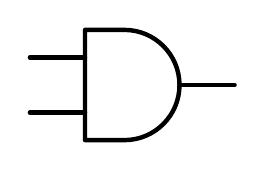
\begin{tikzpicture}[line width=1.6pt, line cap=round, line join=round]
    % Ingressi (linee orizzontali a sinistra)
    \draw (-0.7, 0.35) -- (0, 0.35);
    \draw (-0.7, -0.35) -- (0, -0.35);

    % Corpo della porta AND: lato posteriore dritto, tratti superiore/inferiore e arco semicircolare
    \draw (0, -0.7) -- (0, 0.7) -- (0.5, 0.7) arc[start angle=90, end angle=-90, radius=0.7] -- (0, -0.7);

    % Uscita (linea orizzontale a destra)
    \draw (1.2, 0) -- (1.9, 0);
\end{tikzpicture}
\end{minipage}
\hfill
\begin{minipage}[t]{0.31\textwidth}
    \subsubsection{Descrizione}
    La porta logica AND svolge l'operazione logica di AND tra 2 bit, detta anche prodotto logico
\end{minipage}
\hfill
\begin{minipage}[t]{0.31\textwidth}
        \subsubsection{Tabella}
        \begin{tabular}{|c|c|c|}
            \hline
            $\mathbf{A}$ & $\mathbf{B}$ & $\mathbf{A \cdot B}$ \\ \hline
            0   &   0   &   0 \\ \hline
            0   &   1   &   0 \\ \hline
            1   &   0   &   0 \\ \hline
            1   &   1   &   1 \\ \hline

        \end{tabular}
\end{minipage}


\subsection{Porta logica OR}
\begin{minipage}[t]{0.31\textwidth}
    \subsubsection{Simbolo}
    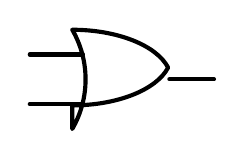
\begin{tikzpicture}[scale=0.9, line width=1.5pt, line cap=round, line join=round]
        % Ingressi (fermati esattamente sul bordo dell'arco)
        \draw (-0.7, 0.35) -- (0.05, 0.35);
        \draw (-0.7, -0.35) -- (0.05, -0.35);
    
        % Corpo della porta OR
        \draw (-0.1, -0.7) 
            arc[start angle=-30, end angle=30, radius=1.4] 
            arc[start angle=90, end angle=15, x radius=1.4, y radius=0.72]
            arc[start angle=-15, end angle=-90, x radius=1.4, y radius=0.72] 
            -- cycle;
    
        % Uscita (attaccata esattamente alla punta)
        \draw (1.27, 0) -- (1.9, 0);
    \end{tikzpicture}
\end{minipage}
\hfil
\begin{minipage}[t]{0.31\textwidth}
    \subsubsection{Descrizione}
    La porta logica OR svolge l'operazione logica di OR tra 2 bit, detta anche somma logica
\end{minipage}
\hfil
\begin{minipage}[t]{0.31\textwidth}
    \subsubsection{Tabella}
    \begin{tabular}{|c|c|c|}
        \hline
        $\mathbf{A}$ & $\mathbf{B}$ & $\mathbf{A+B}$ \\ \hline
        0 & 0 & 0 \\ \hline
        0 & 0 & 0 \\ \hline
        0 & 0 & 0 \\ \hline
        0 & 0 & 0 \\\hline
    \end{tabular}
\end{minipage}

\subsection{Porta logica NOT}
\begin{minipage}[t]{0.31\textwidth}
    \subsubsection{Simbolo}
    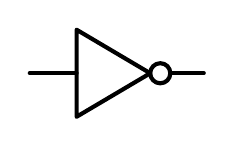
\begin{tikzpicture}[scale=0.85, line width=1.5pt, line cap=round, line join=round]
        % Ingresso
        \draw (-0.7, 0) -- (0, 0);
        % Triangolo
        \draw (0, -0.65) -- (0, 0.65) -- (1.1, 0) -- cycle;
        % Pallino di negazione
        \draw (1.25, 0) circle (0.15);
        % Uscita
        \draw (1.4, 0) -- (1.9, 0);
    \end{tikzpicture}
\end{minipage}
\hfil
\begin{minipage}[t]{0.31\textwidth}
    \subsubsection{Descrizione}
    La porta logica NOT svolge l'operazione logica di not su un bit, detta anche negazione logica
\end{minipage}
\hfil
\begin{minipage}[t]{0.31\textwidth}
    \subsubsection{Tabella}
    \begin{tabular}{|c|c|}
        \hline
        $\mathbf{A}$ & $\mathbf{\overline{A}}$ \\ \hline
        0 & 1 \\ \hline
        1 & 0 \\ \hline
    \end{tabular}
\end{minipage}

\section{Porte logiche derivate}
\subsection{Cosa sono?}
Oltre alle porte logiche fondamentali (AND, OR, NOT) esistono altre porte che sono realizzate combinando le porte fondamentali, il cui principale scopo è la semplificazione dei circuiti (realizzando operazioni composte in un unico componente)

\subsection{Porta logica NAND}
\begin{minipage}[t]{0.31\textwidth}
    \subsubsection{Simbolo}
    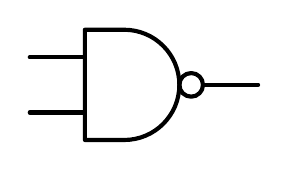
\begin{tikzpicture}[line width=1.5pt, line cap=round, line join=round]
    % Ingressi
    \draw (-0.7, 0.35) -- (0, 0.35);
    \draw (-0.7, -0.35) -- (0, -0.35);

    % Corpo della porta AND
    \draw (0, -0.7) -- (0, 0.7) -- (0.5, 0.7) arc[start angle=90, end angle=-90, radius=0.7] -- cycle;

    % Pallino di negazione (Inversion bubble)
    \draw (1.35, 0) circle (0.15);

    % Uscita
    \draw (1.5, 0) -- (2.2, 0);
\end{tikzpicture}
\end{minipage}
\hfil
\begin{minipage}[t]{0.31\textwidth}
    \subsubsection{Descrizione}
    La porta logica NAND svolge l'operazione logica di NOT sul bit risultante dall'operazione AND sui bit in ingresso
\end{minipage}
\hfil
\begin{minipage}[t]{0.31\textwidth}
    \subsubsection{Tabella}
    \begin{tabular}{|c|c|c|c|}
        \hline
        $\mathbf{A}$ & $\mathbf{B}$ & $\mathbf{A \cdot B}$ & $\mathbf{A \text{ NAND } B}$ \\ \hline
        0 & 0 & 0 & 0 \\ \hline
        0 & 1 & 0 & 0 \\ \hline
        1 & 0 & 0 & 0 \\ \hline
        1 & 1 & 1 & 1 \\ \hline
    \end{tabular}
\end{minipage}

\subsection{Porta logica NOR}
\begin{minipage}[t]{0.31\textwidth}
    \subsubsection{Simbolo}
    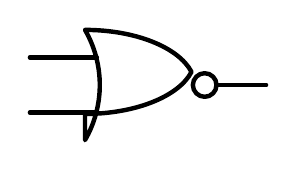
\begin{tikzpicture}[line width=1.6pt, line cap=round, line join=round]

    % Ingressi 
    \draw (-0.8, 0.35) -- (0.05, 0.35);
    \draw (-0.8, -0.35) -- (0.05, -0.35);

    % Corpo della porta OR:
    % 1. Arco concavo posteriore
    % 2. Arco superiore verso la punta destra
    % 3. Arco inferiore di ritorno
    \draw (-0.1, -0.7) 
        arc[start angle=-30, end angle=30, radius=1.4] 
        arc[start angle=90, end angle=15, x radius=1.4, y radius=0.72]
        arc[start angle=-15, end angle=-90, x radius=1.4, y radius=0.72] 
        -- cycle;

    % Pallino di negazione (NOT)
    \draw (1.42, 0) circle (0.15);

    % Uscita a destra
    \draw (1.57, 0) -- (2.2, 0);

\end{tikzpicture}
\end{minipage}
\hfil
\begin{minipage}[t]{0.31\textwidth}
    \subsubsection{Descrizione}
    La porta logica NOR svolge l'operazione logica di NOT sul bit risultante dall'operazione OR sui bit in ingresso
\end{minipage}
\hfil
\begin{minipage}[t]{0.31\textwidth}
    \subsubsection{Tabella}
    \begin{tabular}{|c|c|c|c|}
        \hline $\mathbf{A}$ & $\mathbf{B}$ & $\mathbf{A+B}$ & $\mathbf{A \text{ NOR } B}$ \\ \hline
        0 & 0 & 0 & 1 \\ \hline
        0 & 1 & 1 & 0 \\ \hline
        1 & 0 & 1 & 0 \\ \hline
        1 & 1 & 1 & 0 \\ \hline
    \end{tabular}
\end{minipage}

\newpage
\subsection{Porta logica XOR}
\begin{minipage}[t]{0.31\textwidth}
    \subsubsection{Simbolo}
    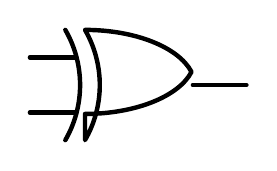
\begin{tikzpicture}[line width=1.6pt, line cap=round, line join=round]

    % Ingressi (linee orizzontali a sinistra che toccano il primo arco)
    \draw (-0.8, 0.35) -- (-0.23, 0.35);
    \draw (-0.8, -0.35) -- (-0.23, -0.35);

    % Arco ricurvo aggiuntivo di ingresso (tipico dello XOR)
    \draw (-0.35, -0.7) arc[start angle=-30, end angle=30, radius=1.4];

    % Corpo della porta OR:
    % 1. Arco concavo posteriore
    % 2. Arco superiore verso la punta destra
    % 3. Arco inferiore di ritorno
    \draw (-0.1, -0.7) 
        arc[start angle=-30, end angle=30, radius=1.4] 
        arc[start angle=90, end angle=15, x radius=1.4, y radius=0.72]
        arc[start angle=-15, end angle=-90, x radius=1.4, y radius=0.72] 
        -- cycle;

    % Uscita (linea orizzontale a destra)
    \draw (1.27, 0) -- (1.95, 0);

\end{tikzpicture}
\end{minipage}
\hfil
\begin{minipage}[t]{0.31\textwidth}
    \subsubsection{Descrizione}
    La porta logica XOR opera come disgiunzione esclusiva tra due input
\end{minipage}
\hfil
\begin{minipage}[t]{0.31\textwidth}
    \subsubsection{Tabella}
    \begin{tabular}{|c|c|c|}
        \hline $\mathbf{A}$ & $\mathbf{B}$ & $\mathbf{A \text{ XOR } B}$ \\ \hline
        0 & 0 & 0 \\ \hline
        0 & 1 & 1 \\ \hline
        1 & 0 & 1 \\ \hline
        1 & 1 & 0 \\ \hline
    \end{tabular}
\end{minipage}

\newpage
\section{Decoder}
\subsection{Cosa è?}
Un decoder è un componente elettronico caratterizzato dall'avere $n$ ingressi e $2^n$ uscite

Lo scopo del decoder è di impostare allo stato alto l'uscita corrispondente alla conversione in base 10 della codifica binaria a $n$ bit ricevuta in input (e di impostare allo stato basso tutte le altre)

\subsection{Come funziona?}
$2^n$ uscite, solo 1 valore è attivo per ogni combinazione di input
\begin{itemize}
    \item L'ingresso seleziona una delle uscite
    \item L'uscita selezionata ha valore 1 tutte le altre 0
\end{itemize}

\vspace{0.5cm}

\begin{minipage}[t]{0.41\textwidth}
    \subsection{Schema semplificato}
    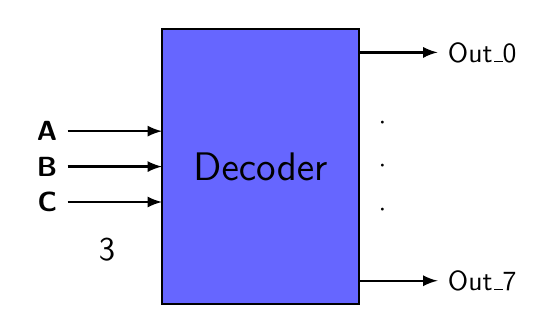
\begin{tikzpicture}[font=\sffamily, >=latex, thick]

        % Corpo del Decoder (rettangolo azzurro)
        \draw[fill=blue!60, draw=black] (0, 0) rectangle (2.5, 3.5);
        \node at (1.25, 1.75) {\Large Decoder};

        % Ingressi a sinistra (A, B, C)
        \draw[->] (-1.2, 2.2) -- (0, 2.2);
        \node[anchor=east] at (-1.2, 2.2) {\textbf{A}};
        
        \draw[->] (-1.2, 1.75) -- (0, 1.75);
        \node[anchor=east] at (-1.2, 1.75) {\textbf{B}};
        
        \draw[->] (-1.2, 1.3) -- (0, 1.3);
        \node[anchor=east] at (-1.2, 1.3) {\textbf{C}};

        % Etichetta "3" sotto le frecce di ingresso
        \node at (-0.7, 0.7) {\large 3};

        % Uscite a destra
        \draw[->] (2.5, 3.2) -- (3.5, 3.2);
        \node[anchor=west] at (3.5, 3.2) {Out\_0};

        % Puntini di sospensione verticali
        \node at (2.8, 2.3) {$\cdot$};
        \node at (2.8, 1.75) {$\cdot$};
        \node at (2.8, 1.2) {$\cdot$};

        \draw[->] (2.5, 0.3) -- (3.5, 0.3);
        \node[anchor=west] at (3.5, 0.3) {Out\_7};

    \end{tikzpicture}
\end{minipage}
\hfil
\begin{minipage}[t]{0.41\textwidth}
    \subsection{Schema dettagliato}
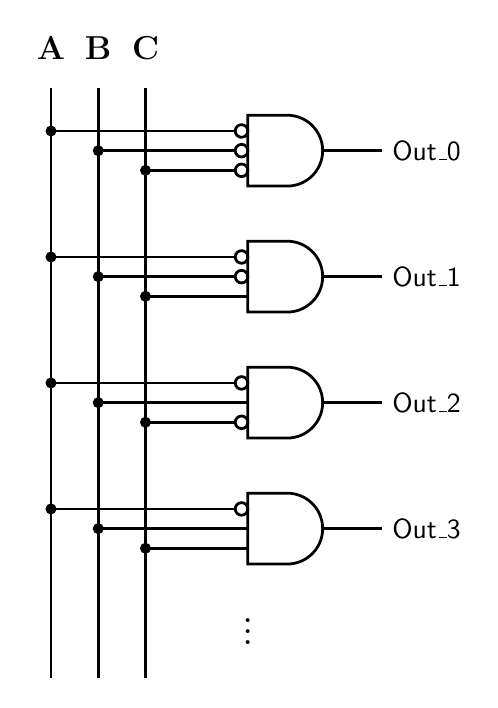
\begin{tikzpicture}[font=\sffamily, line width=1pt, >=latex]

        % ==========================================
        % 1. Linee verticali degli ingressi A, B, C
        % ==========================================
        \node[font=\large\bfseries] at (0, 0.5) {A};
        \node[font=\large\bfseries] at (0.6, 0.5) {B};
        \node[font=\large\bfseries] at (1.2, 0.5) {C};
        
        \draw (0, 0) -- (0, -7.5);
        \draw (0.6, 0) -- (0.6, -7.5);
        \draw (1.2, 0) -- (1.2, -7.5);

        % ==========================================
        % 2. Generazione delle 4 porte logiche AND
        % ==========================================
        % Il ciclo definisce: 
        % \i = indice dell'uscita (0, 1, 2, 3)
        % \invA, \invB, \invC = 1 se c'è il pallino di negazione, 0 se è un filo diretto
        \foreach \i / \invA / \invB / \invC in {
            0/1/1/1, % Out_0: NOT A, NOT B, NOT C
            1/1/1/0, % Out_1: NOT A, NOT B, C
            2/1/0/1, % Out_2: NOT A, B, NOT C
            3/1/0/0  % Out_3: NOT A, B, C
        }{
            % Calcolo la coordinata Y per ogni porta AND (spaziate di 1.6 l'una dall'altra)
            \pgfmathsetmacro{\y}{-0.8 - \i*1.6} 
            
            % Corpo della porta AND
            \draw (2.5, \y-0.45) -- (2.5, \y+0.45) -- (3.0, \y+0.45) arc[start angle=90, end angle=-90, radius=0.45] -- cycle;
            
            % Linea di uscita
            \draw (3.45, \y) -- (4.2, \y) node[right] {Out\_\i};
            
            % --- Collegamento A (ingresso superiore) ---
            \fill (0, \y+0.25) circle (0.07); % Nodo di giunzione sul filo A
            \ifnum\invA=1
                \draw (0, \y+0.25) -- (2.34, \y+0.25);
                \draw (2.42, \y+0.25) circle (0.08); % Pallino di negazione
            \else
                \draw (0, \y+0.25) -- (2.5, \y+0.25);
            \fi

            % --- Collegamento B (ingresso centrale) ---
            \fill (0.6, \y) circle (0.07); % Nodo di giunzione sul filo B
            \ifnum\invB=1
                \draw (0.6, \y) -- (2.34, \y);
                \draw (2.42, \y) circle (0.08);
            \else
                \draw (0.6, \y) -- (2.5, \y);
            \fi

            % --- Collegamento C (ingresso inferiore) ---
            \fill (1.2, \y-0.25) circle (0.07); % Nodo di giunzione sul filo C
            \ifnum\invC=1
                \draw (1.2, \y-0.25) -- (2.34, \y-0.25);
                \draw (2.42, \y-0.25) circle (0.08);
            \else
                \draw (1.2, \y-0.25) -- (2.5, \y-0.25);
            \fi
        }

        % ==========================================
        % 3. Puntini di sospensione finali
        % ==========================================
        \node[font=\Large] at (2.5, -6.8) {$\vdots$};

    \end{tikzpicture}
\end{minipage}

\subsection{Tabella}
{
    \Large

    \begin{center}
        \begin{tabular}{ccc|cccccccc}
            \textbf{A} & \textbf{B} & \textbf{C} & \textbf{0} & \textbf{1} & \textbf{2} & \textbf{3} & \textbf{4} & \textbf{5} & \textbf{6} & \textbf{7} \\
            \hline
            0 & 0 & 0 & $\mathbf{1}$ & 0 & 0 & 0 & 0 & 0 & 0 & 0 \\
            0 & 0 & 1 & 0 & $\mathbf{1}$ & 0 & 0 & 0 & 0 & 0 & 0 \\
            0 & 1 & 0 & 0 & 0 & $\mathbf{1}$ & 0 & 0 & 0 & 0 & 0 \\
            0 & 1 & 1 & 0 & 0 & 0 & $\mathbf{1}$ & 0 & 0 & 0 & 0 \\
            1 & 0 & 0 & 0 & 0 & 0 & 0 & $\mathbf{1}$ & 0 & 0 & 0 \\
            1 & 0 & 1 & 0 & 0 & 0 & 0 & 0 & $\mathbf{1}$ & 0 & 0 \\
            1 & 1 & 0 & 0 & 0 & 0 & 0 & 0 & 0 & $\mathbf{1}$ & 0 \\
            1 & 1 & 1 & 0 & 0 & 0 & 0 & 0 & 0 & 0 & $\mathbf{1}$ \\
        \end{tabular}
    \end{center}
}

\section{Multiplexer}
\subsection{Cosa è?}
Un multiplexer, detto anche selettore, è un componente elettronico caratterizzato da:
\begin{itemize}
    \item $2^n$ entrate principali
    \item $n$ entrate di controllo (selettore)
    \item 1 uscita
\end{itemize}

\subsection{Come funziona?}
In base a quale valore viene immesso nelle entrate di controllo si decide quale valore entrante dalle porte di input verrà portato fuori dal circuito.

Se un multiplexer riceve in input $n$ segnali, esso necessità di $\log_2(n)$ selettori, e consisterà di:
\begin{itemize}
    \item Un decoder che genererà $n$ segnali
    \item Un array di $n$ porte logiche AND
    \item Un'unica porta logica Or
\end{itemize}

\subsection{Esempio}
\begin{minipage}[t]{0.31\textwidth}
    \subsubsection{Schema semplificato}
    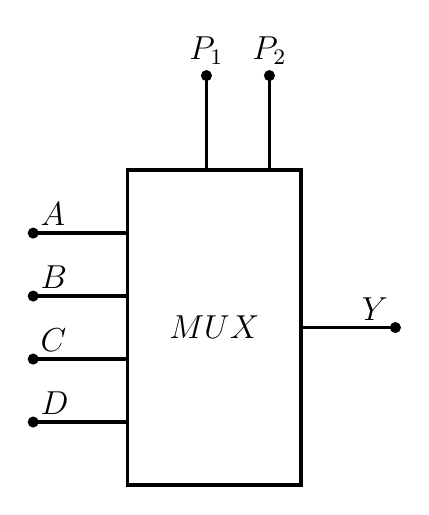
\begin{tikzpicture}[line width=1.3pt, font=\large]

        % --- Corpo del MUX ---
        % Disegna il rettangolo principale
        \draw (0, 0) rectangle (2.2, 4);
        % Testo centrale
        \node at (1.1, 2) {$MUX$};

        % --- Ingressi a sinistra (A, B, C, D) ---
        % Linee di ingresso e pallini
        \foreach \y/\label in {3.2/A, 2.4/B, 1.6/C, 0.8/D} {
            \draw (-1.2, \y) -- (0, \y);
            \fill (-1.2, \y) circle (2pt);
            % Etichette posizionate sopra le linee, vicino al pallino
            \node[above right, inner sep=2pt] at (-1.2, \y) {$\label$};
        }

        % --- Ingressi di selezione in alto (P1, P2) ---
        % P1
        \draw (1.0, 4) -- (1.0, 5.2);
        \fill (1.0, 5.2) circle (2pt);
        \node[above] at (1.0, 5.2) {$P_1$};

        % P2
        \draw (1.8, 4) -- (1.8, 5.2);
        \fill (1.8, 5.2) circle (2pt);
        \node[above] at (1.8, 5.2) {$P_2$};

        % --- Uscita a destra (Y) ---
        \draw (2.2, 2) -- (3.4, 2);
        \fill (3.4, 2) circle (2pt);
        % Etichetta posizionata sopra la linea, prima del pallino
        \node[above left, inner sep=2pt] at (3.4, 2) {$Y$};

    \end{tikzpicture}
\end{minipage}
\hfil
\begin{minipage}[t]{0.31\textwidth}
    \subsubsection{Schema dettagliato}
    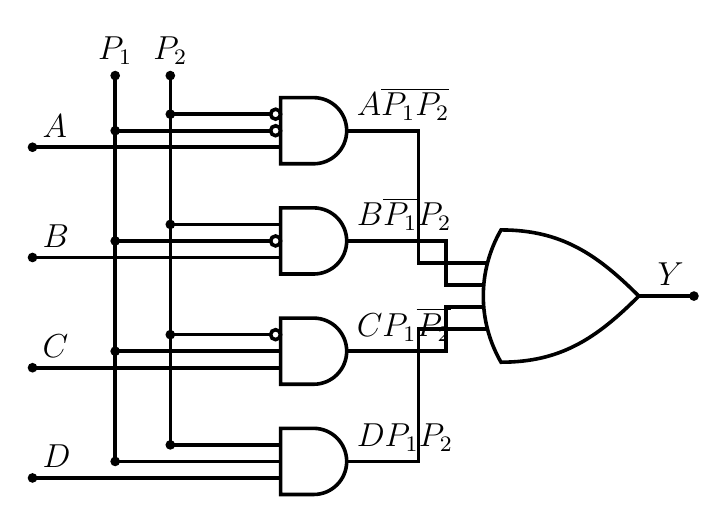
\begin{tikzpicture}[font=\large, line width=1.3pt, >=latex, scale=0.7]

        % --- Linee verticali dei segnali di selezione (P1, P2) ---
        % P1
        \draw (1.0, 4.5) -- (1.0, -2.5);
        \fill (1.0, 4.5) circle (2.5pt);
        \node[above] at (1.0, 4.5) {$P_1$};

        % P2
        \draw (2.0, 4.5) -- (2.0, -2.2);
        \fill (2.0, 4.5) circle (2.5pt);
        \node[above] at (2.0, 4.5) {$P_2$};

        % --- Generazione automatizzata delle 4 porte AND ---
        % \i = indice, \y = quota verticale, \lbl = Input, \invPone = negazione P1, \invPtwo = negazione P2, \outText = etichetta uscita
        \foreach \i / \y / \lbl / \invPone / \invPtwo / \outText in {
            0 /  3.5 / A / 1 / 1 / A\overline{P_1}\overline{P_2},
            1 /  1.5 / B / 1 / 0 / B\overline{P_1}P_2,
            2 / -0.5 / C / 0 / 1 / CP_1\overline{P_2},
            3 / -2.5 / D / 0 / 0 / DP_1P_2
        } {
            % 1. Corpo della porta AND
            \draw[fill=white] (4.0, \y-0.6) -- (4.0, \y+0.6) -- (4.6, \y+0.6) 
                arc[start angle=90, end angle=-90, radius=0.6] -- cycle;
            
            % 2. Ingresso Dati (A, B, C, D) - Pin inferiore
            \draw (-0.5, \y-0.3) -- (4.0, \y-0.3);
            \fill (-0.5, \y-0.3) circle (2.5pt);
            \node[above right, inner sep=3pt] at (-0.5, \y-0.3) {$\lbl$};

            % 3. Ingresso di selezione P1 - Pin centrale
            \fill (1.0, \y) circle (2.5pt);
            \ifnum\invPone=1
                \draw (1.0, \y) -- (3.82, \y);
                \draw (3.91, \y) circle (0.09); % Pallino di negazione
            \else
                \draw (1.0, \y) -- (4.0, \y);
            \fi

            % 4. Ingresso di selezione P2 - Pin superiore
            \fill (2.0, \y+0.3) circle (2.5pt);
            \ifnum\invPtwo=1
                \draw (2.0, \y+0.3) -- (3.82, \y+0.3);
                \draw (3.91, \y+0.3) circle (0.09); % Pallino di negazione
            \else
                \draw (2.0, \y+0.3) -- (4.0, \y+0.3);
            \fi

            % 5. Etichetta del Mintermine in uscita dalla porta AND
            \node[above right, inner sep=3pt] at (5.2, \y) {$\outText$};
        }

        % --- Collegamenti dalle uscite AND verso la porta OR centrale ---
        % Sfruttiamo la simmetria convogliandole verso il centro a y=0.5
        
        % AND 1 (da y=3.5 scende a y=1.1)
        \draw (5.2, 3.5) -- (6.5, 3.5) -- (6.5, 1.1) -- (7.9, 1.1);
        % AND 2 (da y=1.5 scende a y=0.7)
        \draw (5.2, 1.5) -- (7.0, 1.5) -- (7.0, 0.7) -- (7.9, 0.7);
        % AND 3 (da y=-0.5 sale a y=0.3)
        \draw (5.2, -0.5) -- (7.0, -0.5) -- (7.0, 0.3) -- (7.9, 0.3);
        % AND 4 (da y=-2.5 sale a y=-0.1)
        \draw (5.2, -2.5) -- (6.5, -2.5) -- (6.5, -0.1) -- (7.9, -0.1);

        % --- Porta OR di uscita ---
        % Disegnata sfruttando curve di Bezier native centrate in y=0.5
        % Il fill=white copre gli estremi delle linee in ingresso in modo pulito
        \draw[fill=white] (8.0, 1.7) arc[start angle=150, end angle=210, radius=2.4] 
            to[out=0, in=225] (10.5, 0.5) 
            to[out=135, in=0] cycle;

        % --- Uscita finale Y ---
        \draw (10.5, 0.5) -- (11.5, 0.5);
        \fill (11.5, 0.5) circle (2.5pt);
        \node[above left, inner sep=3pt] at (11.5, 0.5) {$Y$};

    \end{tikzpicture}
\end{minipage}


\subsubsection{Tabella}
\noindent
\begin{minipage}[t]{0.2\textwidth}
   {
    \LARGE
    \vspace{0pt} % Fissa l'allineamento in cima
    \centering
    \begin{tabular}{cc|c}
        $P_1$ & $P_2$ & $Y$ \\
        \hline
        0 & 0 & $A$ \\
        0 & 1 & $B$ \\
        1 & 0 & $C$ \\
        1 & 1 & $D$ \\
    \end{tabular}}
\end{minipage}%
\hfill
\begin{minipage}[t]{0.7\textwidth}
    \subsubsection{}
    \vspace{-1.5em} % Sposta la formula più in alto (regola a piacimento)
    {
        \LARGE
        \begin{equation*}
        Y = A\overline{P_1}\overline{P_2} + B\overline{P_1}P_2 + CP_1\overline{P_2} + DP_1P_2
    \end{equation*}}
\end{minipage}

\section{PLA - Programmable Logic Array}
\subsection{Cosa è?}
La somma di prodotti corrisponde ad una implementazione comunemente nota come Programmable Logic Array (PLA)

\subsection{Da cosa è compasta?}
\begin{itemize}
    \item Un insieme di input
    \item I corrispondenti input complementanti (mediante inverter) per poter gestire più uscite
    \item Una logica a 2 stage:
    \begin{enumerate}
        \item Un array di prote logiche AND
        \item Un array di porte logiche OR
    \end{enumerate}
\end{itemize}

\subsection{Esempio}

\begin{minipage}[t]{0.45\textwidth}
    \subsubsection{Schema semplificato}
    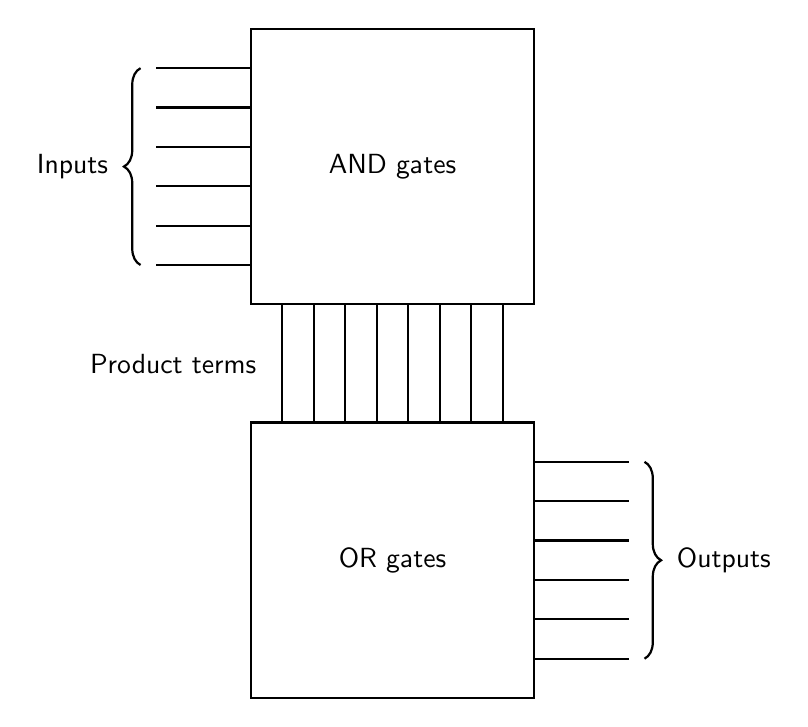
\begin{tikzpicture}[font=\sffamily, thick]

        % ==========================================
        % 1. Blocchi Principali (AND e OR gates)
        % ==========================================
        \draw (0, 0) rectangle (3.6, 3.5);
        \node at (1.8, 1.75) {AND gates};

        \draw (0, -1.5) rectangle (3.6, -5.0);
        \node at (1.8, -3.25) {OR gates};

        % ==========================================
        % 2. Ingressi (Sinistra)
        % ==========================================
        % 6 linee orizzontali di ingresso
        \foreach \y in {0.5, 1.0, 1.5, 2.0, 2.5, 3.0} {
            \draw (-1.2, \y) -- (0, \y);
        }
        % Parentesi graffa e testo "Inputs"
        \draw [decorate, decoration={brace, amplitude=6pt}] 
            (-1.4, 0.5) -- (-1.4, 3.0) node [midway, left=8pt] {Inputs};

        % ==========================================
        % 3. Product terms (Connessioni centrali)
        % ==========================================
        % 8 linee verticali tra il blocco AND e il blocco OR
        \foreach \x in {0.4, 0.8, 1.2, 1.6, 2.0, 2.4, 2.8, 3.2} {
            \draw (\x, 0) -- (\x, -1.5);
        }
        % Etichetta laterale per i Product terms
        \node[anchor=east] at (0.2, -0.75) {Product terms};

        % ==========================================
        % 4. Uscite (Destra)
        % ==========================================
        % 6 linee orizzontali di uscita
        \foreach \y in {-2.0, -2.5, -3.0, -3.5, -4.0, -4.5} {
            \draw (3.6, \y) -- (4.8, \y);
        }
        % Parentesi graffa e testo "Outputs"
        \draw [decorate, decoration={brace, amplitude=6pt}] 
            (5.0, -2.0) -- (5.0, -4.5) node [midway, right=8pt] {Outputs};

    \end{tikzpicture}
\end{minipage}
\hfil
\begin{minipage}[t]{0.45\textwidth}
    \subsubsection{Tabella}
        \begin{center}
            \begin{tabular}{|c|c|c|c|c|c|}
                \hline
                \multicolumn{3}{|c|}{\textbf{Inputs}} & \multicolumn{3}{c|}{\textbf{Outputs}} \\
                \hline
                \textbf{A} & \textbf{B} & \textbf{C} & \textbf{D} & \textbf{E} & \textbf{F} \\
                \hline
                0 & 0 & 0 & 0 & 0 & 0 \\
                \hline
                0 & 0 & 1 & 1 & 0 & 0 \\
                \hline
                0 & 1 & 0 & 1 & 0 & 0 \\
                \hline
                0 & 1 & 1 & 1 & 1 & 0 \\
                \hline
                1 & 0 & 0 & 1 & 0 & 0 \\
                \hline
                1 & 0 & 1 & 1 & 1 & 0 \\
                \hline
                1 & 1 & 0 & 1 & 1 & 0 \\
                \hline
                1 & 1 & 1 & 1 & 0 & 1 \\
                \hline
            \end{tabular}
    \end{center}
\end{minipage}

\subsubsection{Schema dettagliato}
\begin{center}
    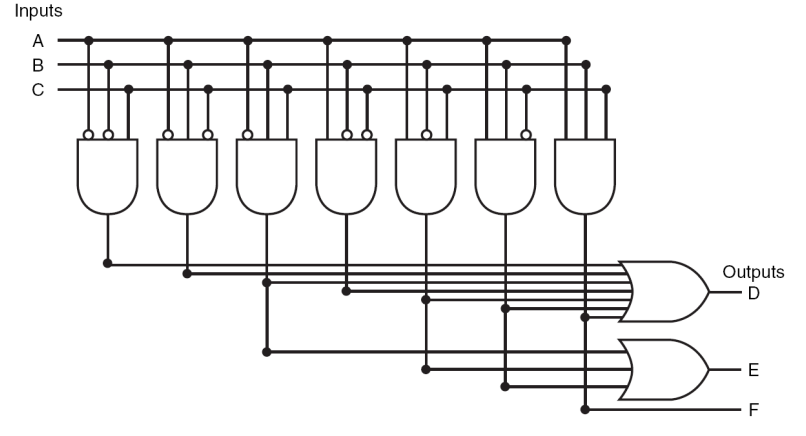
\includegraphics[scale=0.65]{Immagini/Schema PLA.png}
\end{center}
\subsubsection{Formula dell'esempio}

{
    \Large
    \begin{gather*}
        D = \overline{AB}C + \overline{A}B\overline{C} + \overline{A}BC + A\overline{BC} + A\overline{B}C + AB\overline{C} + ABC \\
        E = \overline{A}BC + A\overline{B}C + AB\overline{C} \\
        F = ABC
    \end{gather*}
}


\newpage
\section{Array di elementi logici}
\subsection{Cosa sono?}
La maggior parte delle operazioni vengono svolte su 32 bit, mettendo in luce la necessità di creare array di elementi logici, ossia un bus, una collezione di linee di input che verranno trattate come un singolo segnale

\subsection{Esempio con Multiplexer a 32 bit}
    \begin{minipage}[t]{0.45\textwidth}
    \subsubsection{Schema semplificato}
        \begin{center}
            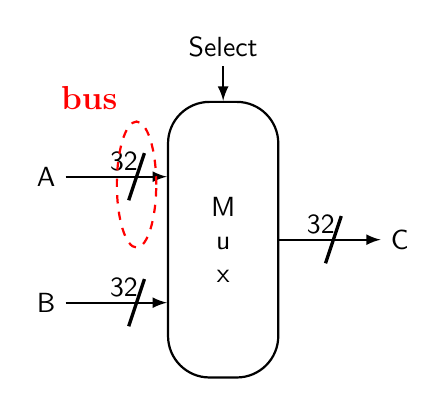
\begin{tikzpicture}[
                font=\sffamily,
                thick,
                >=latex,
                % Stile per il corpo del Multiplexer
                mux/.style={
                    draw,
                    rounded corners=15pt,
                    minimum width=1.4cm,
                    minimum height=3.5cm,
                    align=center,
                    inner sep=0pt
                }
            ]

                % --- Corpo centrale (Mux) ---
                \node[mux] (M) at (0,0) {M\\u\\x};

                % --- Ingresso A (Superiore) ---
                \draw[->] (-2.0, 0.8) node[left] {A} -- (M.west |- 0,0.8);
                % Taglio bus e "32"
                \draw[line width=1.2pt] (-1.2, 0.5) -- (-1.0, 1.1);
                \node[above left, inner sep=2pt] at (-1.0, 0.8) {32};

                % Evidenziatore rosso tratteggiato (bus)
                \draw[red, dashed] (-1.1, 0.7) ellipse (0.25cm and 0.8cm);
                \node[red, font=\bfseries\large] at (-1.7, 1.8) {bus};

                % --- Ingresso B (Inferiore) ---
                \draw[->] (-2.0, -0.8) node[left] {B} -- (M.west |- 0,-0.8);
                % Taglio bus e "32"
                \draw[line width=1.2pt] (-1.2, -1.1) -- (-1.0, -0.5);
                \node[above left, inner sep=2pt] at (-1.0, -0.8) {32};

                % --- Segnale di Selezione (Select) ---
                \draw[->] (0, 2.2) node[above] {Select} -- (M.north);

                % --- Uscita C ---
                \draw[->] (M.east) -- (2.0, 0) node[right] {C};
                % Taglio bus e "32"
                \draw[line width=1.2pt] (1.3, -0.3) -- (1.5, 0.3);
                \node[above left, inner sep=2pt] at (1.5, 0) {32};

            \end{tikzpicture}
        \end{center}
    \end{minipage}
    \hfil
    \begin{minipage}[t]{0.45\textwidth}
        \subsubsection{Schema dettagliato}
        \begin{center}
            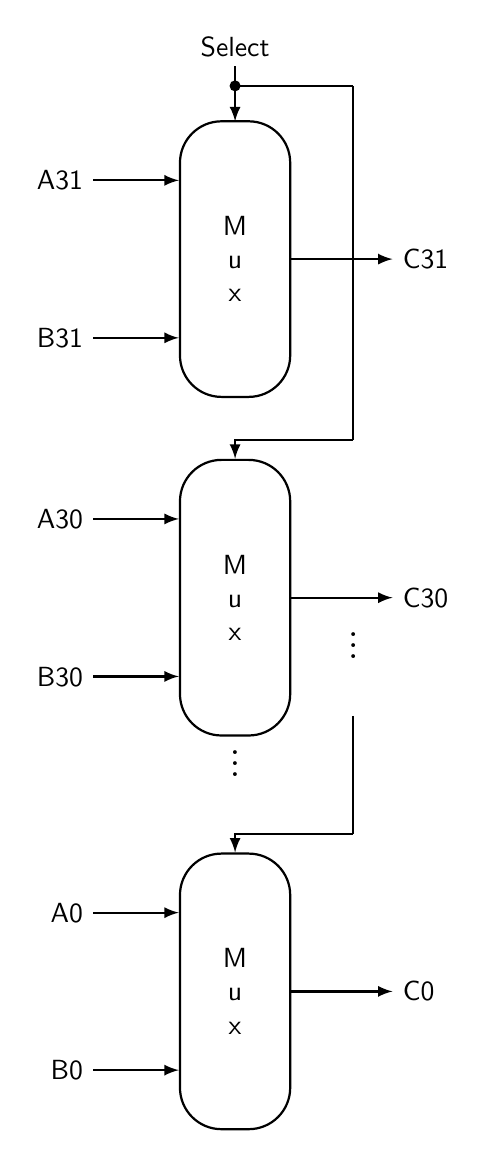
\begin{tikzpicture}[
                font=\sffamily,
                thick,
                >=latex,
                % Stile per i Multiplexer (forma ovale allungata)
                mux/.style={
                    draw,
                    rounded corners=15pt,
                    minimum width=1.4cm,
                    minimum height=3.5cm,
                    align=center
                }
            ]

                % ========================================================
                % 1. Nodo di selezione globale (in alto)
                % ========================================================
                \node (select_top) at (0, 7.5) {Select};
                
                % Nodo (pallino) di derivazione
                \fill (0, 7.0) circle (2pt);
                
                % Freccia verso il primo Mux
                \draw[->] (select_top) -- (0, 7.0) -- (0, 6.55);
                
                % Linea orizzontale che va verso destra per scendere lungo la cascata
                \draw (0, 7.0) -- (1.5, 7.0); 

                % ========================================================
                % 2. MUX Superiore (Bit 31)
                % ========================================================
                \node[mux] (mux31) at (0, 4.8) {M\\u\\x};
                
                % Ingressi A31 e B31
                \draw[->] (-1.8, 5.8) node[left] {A31} -- (mux31.west |- 0, 5.8);
                \draw[->] (-1.8, 3.8) node[left] {B31} -- (mux31.west |- 0, 3.8);
                
                % Uscita C31
                \draw[->] (mux31.east) -- (2.0, 4.8) node[right] {C31};

                % Linea della cascata Select che scende fino al livello del secondo MUX
                \draw (1.5, 7.0) -- (1.5, 2.5);


                % ========================================================
                % 3. MUX Centrale (Bit 30)
                % ========================================================
                \node[mux] (mux30) at (0, 0.5) {M\\u\\x};
                
                % Ingressi A30 e B30
                \draw[->] (-1.8, 1.5) node[left] {A30} -- (mux30.west |- 0, 1.5);
                \draw[->] (-1.8, -0.5) node[left] {B30} -- (mux30.west |- 0, -0.5);
                
                % Uscita C30
                \draw[->] (mux30.east) -- (2.0, 0.5) node[right] {C30};

                % Select ingresso per MUX 30 (curva da destra verso il centro in alto)
                \draw[->] (1.5, 2.5) -- (0, 2.5) -- (mux30.north);


                % ========================================================
                % 4. Puntini di Sospensione
                % ========================================================
                % Puntini verticali tra Mux 30 e Mux 0
                \node[font=\Large] at (0, -1.5) {$\vdots$};
                
                % Puntini per la linea del Select
                \node[font=\Large] at (1.5, 0) {$\vdots$}; 

                % Continuazione linea select verso il basso
                \draw (1.5, -1.0) -- (1.5, -2.5);


                % ========================================================
                % 5. MUX Inferiore (Bit 0)
                % ========================================================
                \node[mux] (mux0) at (0, -4.5) {M\\u\\x};
                
                % Ingressi A0 e B0
                \draw[->] (-1.8, -3.5) node[left] {A0} -- (mux0.west |- 0, -3.5);
                \draw[->] (-1.8, -5.5) node[left] {B0} -- (mux0.west |- 0, -5.5);
                
                % Uscita C0
                \draw[->] (mux0.east) -- (2.0, -4.5) node[right] {C0};

                % Select ingresso per MUX 0
                \draw[->] (1.5, -2.5) -- (0, -2.5) -- (mux0.north);

            \end{tikzpicture}
        \end{center}
    \end{minipage}
